\section{Library design and implementation}
The previous chapter focused on the domain decomposition method and how to model the underlying source graph for stencil codes.
However, domain decomposition is only the initial part of this automated domain decomposition library for stencil codes.
Once the domain is decomposed additional functionalities need to be provided to make a stencil code run on a decomposed domain.

Conceptually the library can be separated into three distinct parts:
Pre-process, runtime, and post-process.
The flowchart in figure \ref{fig:library_flowchart} gives an abstract overview of the whole automatic domain decomposition process.

\begin{figure}
\centering
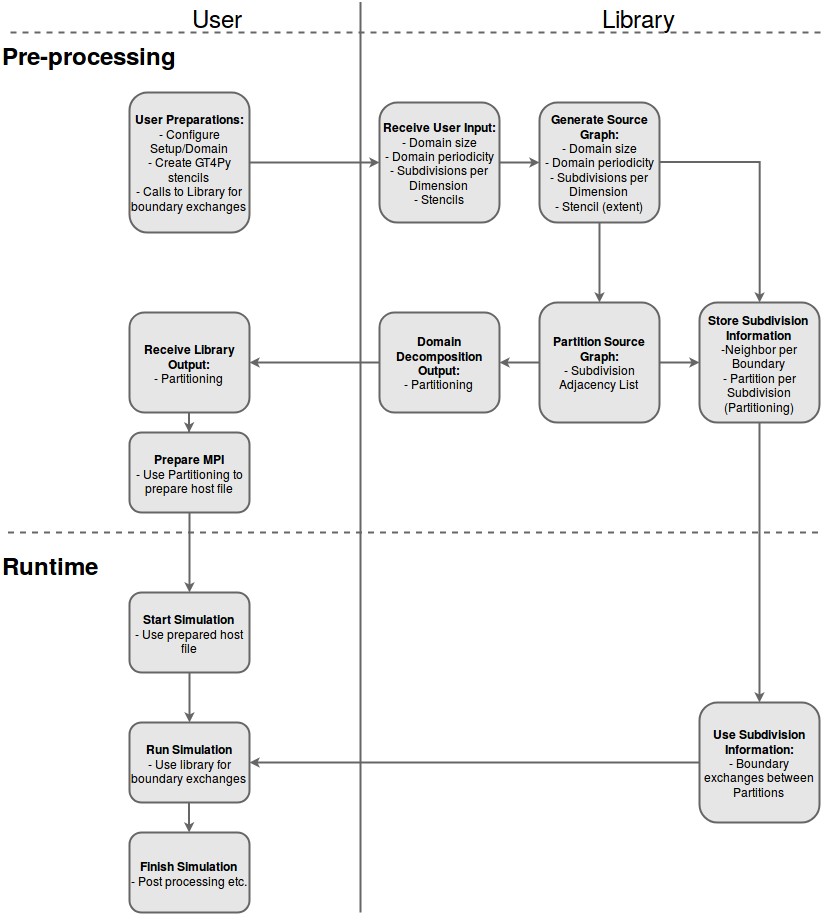
\includegraphics[width=\textwidth]{ddflowchart.png}
\caption{Schematic description of the flow for the automatic domain decomposition process.}
\label{fig:library_flowchart}
\end{figure}

The next sections will first outline the design and functionality of each of these three parts and then show and explain the user facing functions in more detail with examples.

\subsection{Design}
% TODO small intro / abstract design goals 
\subsubsection{Pre-process}
The pre-process contains functionalities needed before the main, distributed stencil computations are performed.
Specifically, the actual domain decomposition happens during the pre-process.
Therefore the pre-process contains functions to prepare the graph partitioning files, perform the actual graph partitioning, and store the results.

The implementation of the pre-process functions follows the descriptions of the source graph generation, and graph partitioning from the previous chapter in the sections \ref{sec:commcost}, \ref{sec:compcost}, and \ref{sec:sourcegraphgeneration} and the pseudo-code of alg. \ref{alg:domaindecomposition} very closely.

The user-facing part of the pre-process implementation is outlined with examples in section \ref{sec:userpreprocess}.

\subsubsection{Runtime process}
% TODO Main functionalities / internal boundary exchanges local / external / global boundary etc




\begin{figure}
\centering
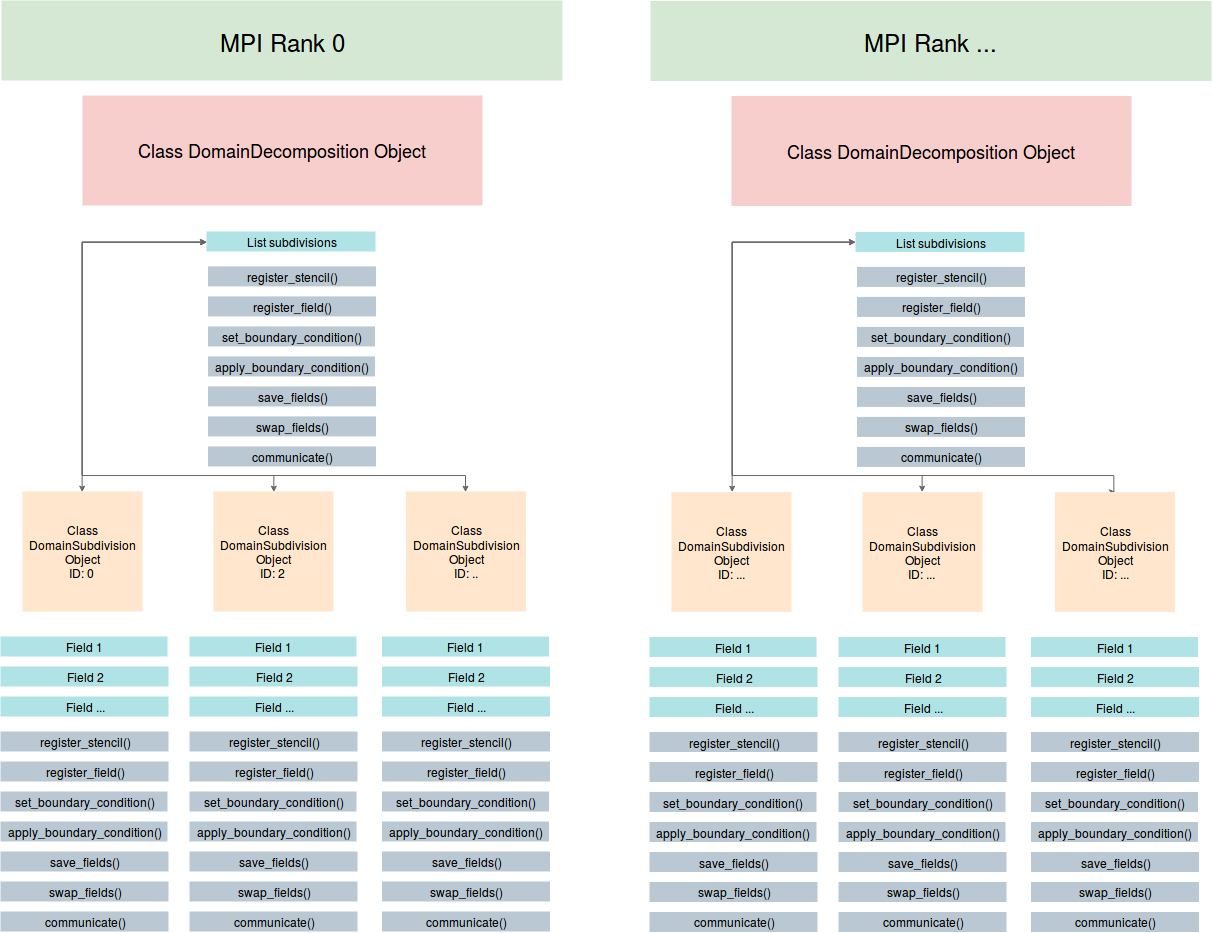
\includegraphics[width=\textwidth]{Classes_Delegation.png}
\caption{Overview.}
\label{fig:classes_chart}
\end{figure}

\subsubsection{Post-process}
% TODO mainly combining field data from various subdivisions back into one file

\begin{figure}
\centering
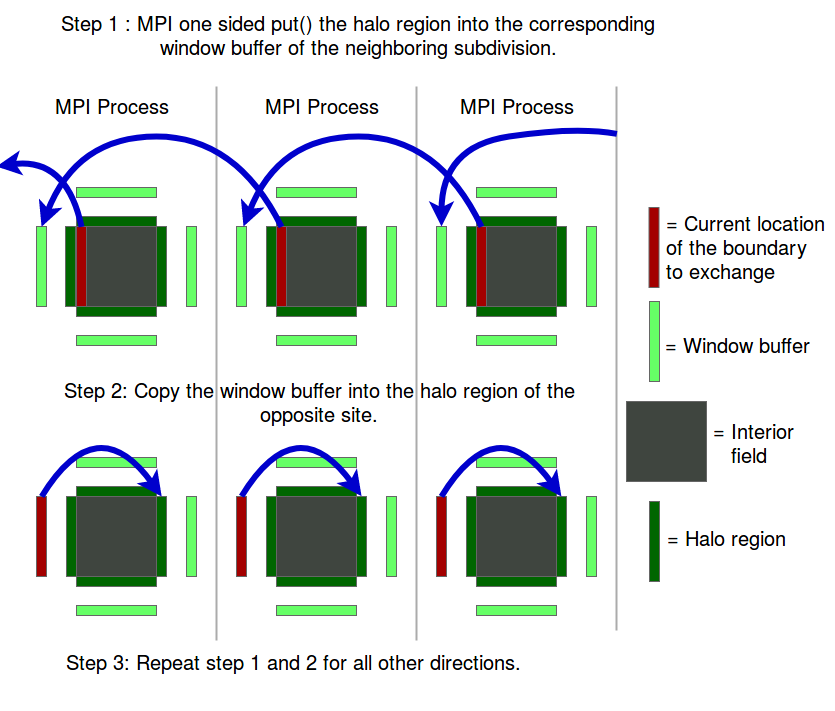
\includegraphics[width=\textwidth]{mpi_onesided.png}
\caption{Overview.}
\label{fig:mpi_onesided_communication_flow}
\end{figure}

\newpage
\subsection{User interface}
The following subsections go through the additional code and code modifications required to transform a non-distributed gridtools code into a domain decomposed and distributed gridtools code.

\subsubsection{Pre-process: Additional setup information.}
\label{sec:userpreprocess}
To start the domain decomposition pre-process the \texttt{DomainPreprocess} class needs to be initialized with the size of the computational domain, the periodicity of the global boundary, and the number of subdivisions per dimension.
Optionally, the path and prefix arguments can be provided to store all the files under the given path and using the given prefix.

Additionally the domain decomposition method needs as user input the access pattern of the stencils used.
The stencil patterns are added by calling the \texttt{add\_stencil()} function of the \texttt{DomainPreprocess} class.
The \texttt{add\_stencil()} needs as input a Python dict with the name of the field as the key and a list of size 6 as the item.
The list of size 6 contains the access pattern list for each direction.

The first entry in the list corresponds to the access pattern in the negative x-direction.
The second entry corresponds to the positive x-direction.
The third entry corresponds to the negative y-direction, then the 4th is the positive y-direction, followed by the negative z-direction and lastly the positive z-direction.

The access patterns themselves are lists of indices that the stencil accesses in that direction.
For example the simple two dimensional Laplace stencil would have a list that looks like this: \texttt{[[1], [1], [1], [1], [0], [0]]}

After all stencils are added this way the actual domain decomposition can be done by calling the \texttt{preprocess()} function of the \texttt{DomainPreprocess} class.
This function generates the graph to be partitioned and saves the subdivision information in a pickle file.

Lastly, the \texttt{pymetis\_partitioning(nparts)} function of the \texttt{DomainPreprocess} class can be called to generate the partitioning. The input argument \texttt{nparts} is the number of partitions that should be generated.

Listing \ref{alg:domainpreprocess} shows a full example for this pre-process user code.

\begin{lstlisting}[caption={Example code of the domain pre-process function calls and additional information needed to decompose a domain.},captionpos=b, label={alg:domainpreprocess}, float, floatplacement=H]
ddc = DomainPreprocess(domain=cdomain, periodic=periodic, subdivs_per_dim=slices, path=path, prefix=prefix)

# Add Use case specific stencils:
if method == 'forward_backward':
    ddc.add_stencil({"unow": [[1], [1], [1], [1], [0], [0]]})
    ddc.add_stencil({"vnow": [[1], [1], [1], [1], [0], [0]]})
elif method == 'upwind':
    ddc.add_stencil({"unow": [[1], [1], [1], [1], [0], [0]]})
    ddc.add_stencil({"vnow": [[1], [1], [1], [1], [0], [0]]})
elif method == 'upwind_third_order':
    ddc.add_stencil({"unow": [[2], [2], [2], [2], [0], [0]]})
    ddc.add_stencil({"vnow": [[2], [2], [2], [2], [0], [0]]})

# Once all stencils are added call preprocess and partitioning
ddc.preprocess()
ddc.pymetis_partitioning(nparts)
\end{lstlisting}

\subsubsection{Pre-process: Initialization of fields.}
Before the any stencil computation can start the initial values of the fields need to be provided.
In simple, serial codes this can be done just before the time stepping.
However, for the distributed parallel code it is simpler and better to store the initial values of the fields in files during the pre-process.
This is simpler, because all distributed nodes will need access to their parts of the fields.
Therefore, if the initial conditions were set during the runtime, either each subdivision would need to initialize its field or a centralized initialization would need to be sent to each subdivision.
Distributing the initialization to each subdivision can become complicated for initial conditions that depend on their position in the global domain.
Initializing centrally and sending the initial values out can become a bottleneck for large domains, if the global domain needs more memory than a single node can provide.

Therefore, at least at the moment the domain decomposition library uses Numpy files generated in the pre-process for initialization of the fields.

An example for this field initialization can be viewed in listing \ref{alg:initfields}.

\begin{lstlisting}[caption={Example code of the domain pre-process function to initialize to fields "unew" and "vnew"},captionpos=b, label={alg:initfields}, float, floatplacement=H]
def prepare_initial_condition(nx, ny, nz, dxs, dxe, dys, dye, nb):
        domain = [(dxs, dys), (dxe, dye)]
        datatype = np.float64

        # Create the grid
        x = np.linspace(domain[0][0], domain[1][0], nx - 2 * nb)
        y = np.linspace(domain[0][1], domain[1][1], ny - 2 * nb)

        # Instatiate the arrays representing the solution
        unew = np.zeros((nx, ny, 1), dtype=datatype)
        vnew = np.zeros((nx, ny, 1), dtype=datatype)

        # Set the initial conditions
        for i in range(nb, nx - nb):
            for j in range(nb, ny - nb):
                if (0.5 <= x[i - nb] and x[i - nb] <= 1.0) and (0.5 <= y[j - nb] and y[j - nb] <= 1.0):
                    unew[i, j, 0], vnew[i, j, 0] = 0.0, 1.0
                else:
                    unew[i, j, 0], vnew[i, j, 0] = 1.0, 0.0

        # Apply the boundary conditions
        unew[0, :, 0], vnew[0, :, 0] = 0., 0.
        unew[-1, :, 0], vnew[-1, :, 0] = 0., 0.
        unew[:, 0, 0], vnew[:, 0, 0] = 0., 0.
        unew[:, -1, 0], vnew[:, -1, 0] = 0., 0.

        np.save(path + prefix + "shankar_initial_conditions_unew.npy", unew)
        np.save(path + prefix + "shankar_initial_conditions_vnew.npy", vnew)
\end{lstlisting}

\subsubsection{Main: Loading domain decomposition information.}
The main or runtime code needs to be modified in a few places to change a serial code to use the domain decomposition library.

The first change is initializing the \texttt{DomainDecomposition} class and loading the subdivision information and domain partitioning generated in the pre-process.

The \texttt{DomainDecomposition} class needs the name of the partitioning file and the format of the partitioning (i.e. either "metis" or "scotch") as input arguments.
Optionally, the same path and prefix arguments as in the pre-process have to be provided if the files are stored under the given path and using the given prefix.

The subdivision information file uses the name generated in the pre-process and therefore does not need to be provided by the user.

The listing \ref{alg:infoload} shows such an initialization call.

\begin{lstlisting}[caption={Example code for the loading of the domain decomposition information.},captionpos=b, label={alg:infoload}, float, floatplacement=H]
prep_domain = DomainDecomposition("subdomains_pymetis.dat.part.4", "metis", path=path, prefix=prefix)
\end{lstlisting}

\subsubsection{Main: Instantiation of fields.}
The instantiation of the fields used by the stencil computations needs to be modified for the use with the domain decomposition library.

Usually in the serial code field instantiation corresponds to a single call to \texttt{numpy.zeros} before the initial conditions are applied.

For the domain decomposition library the fields need to be registered with call to the \texttt{register\_field()} function of the \texttt{DomainDecomposition} class.

The fields need to be registered in this way because the separate subdivision need to instantiate their own Numpy array of the field instead of a global array for each field.

Registering the fields to the \texttt{DomainDecomposition} class requires the name of the field, the extent of the halo of the field, and the initial value file generated in the pre-process.

The extent of the halo is a list of size 6 were each entry corresponds to one direction and the value is the largest offset in that direction.
The order is the same as for the stencil access pattern in the pre-process i.e. negative x-direction, positive x-direction, negative y-direction, positive y-direction, negative z-direction, and positive z-direction.
But in contrast to the stencil access pattern the field halos only need the maximum of the stencil offsets in each direction and not every access.

The field halo extent here are needed to instantiate fields in the subdivisions in the correct size since they have to contain the interior cells corresponding to the solution as well as the halos to each of their neighbors used in the boundary exchanges.

Listing \ref{alg:refinstant} and listing \ref{alg:ddinstant} show the direct comparison between the original instantiation of four fields and the corresponding registration process needed in the domain decomposition library.
This should demonstrate that code needed to be added by the user is kept to a minimum.

\begin{lstlisting}[caption={Example code for the original user field instantiation.},captionpos=b, label={alg:refinstant}, float, floatplacement=H]
# Instantiate the arrays representing the solution
unow = np.zeros((nx, ny, 1), dtype = datatype)
unew = np.zeros((nx, ny, 1), dtype = datatype)
vnow = np.zeros((nx, ny, 1), dtype = datatype)
vnew = np.zeros((nx, ny, 1), dtype = datatype)
\end{lstlisting} 

\begin{lstlisting}[caption={Example code for the same field instantiation using the domain decomposition library.},captionpos=b, label={alg:ddinstant}, float, floatplacement=H]
halo = [1, 1, 1, 1, 0, 0]
prep_domain.register_field(fieldname="unow", halo=halo, field_ic_file=path + prefix +"shankar_initial_conditions_unew.npy")

prep_domain.register_field(fieldname="vnow", halo=halo, field_ic_file=path + prefix +"shankar_initial_conditions_vnew.npy")

prep_domain.register_field(fieldname="unew", halo=halo, field_ic_file=path + prefix +"shankar_initial_conditions_unew.npy")

prep_domain.register_field(fieldname="vnew", halo=halo, field_ic_file=path + prefix +"shankar_initial_conditions_vnew.npy")
\end{lstlisting}

\subsubsection{Main: Instantiation of stencils.}
A small code modification is also necessary for the instantiation of the stencils.
While in serial code the stencils can be directly instantiated by a call to gridtools python module in the domain decomposition libary version the stencil needs to be registered to the \texttt{DomainDecomposition} class instead.

As with the field registration this is due to distributed nature of the domain decomposition library.
Each subdivision needs its own gridtools stencil to use for their computations.

However, for stencil instantiation the code modifications needed are very minimal.
Listing \ref{alg:refstencil} compared to listing \ref{alg:ddstencil} show that the only adjustments needed are the function call from \texttt{gt.NGStencil()} to \texttt{"DomainDecompositionInstance".register\_stencil()} and for each field in the inputs and outputs instead of directly providing the numpy arrays registering their names.

Also, note that the \texttt{domain} keyword can be dropped, since the subdivisions need to define their domain based on the halos provided in field registration.

\begin{lstlisting}[caption={Example code for the original user stencil instantiation.},captionpos=b, label={alg:refstencil}, float, floatplacement=H]
# Instantiate stencil object
stencil = gt.NGStencil(
    definitions_func = definitions_func_,
    inputs = {'in_u': unow, 'in_v': vnow},
    global_inputs = {'dt': dt_, 'dx': dx_, 'dy': dy_, 'eps': eps_},
    outputs = {'out_u': unew, 'out_v': vnew},
    domain = domain_,
    mode = gt.mode.NUMPY
    )
\end{lstlisting}

\begin{lstlisting}[caption={Example code for the same stencil instantiation using the domain decomposition library.},captionpos=b, label={alg:ddstencil}, float, floatplacement=H]
# Instantiate stencil object
stencil = prep_domain.register_stencil(
    definitions_func=definitions_func_,
    inputs={'in_u': "unow", 'in_v': "vnow"},
    global_inputs={'dt': dt_, 'dx': dx_, 'dy': dy_, 'eps': eps_},
    outputs={'out_u': "unew", 'out_v': "vnew"},
    mode=gt.mode.NUMPY
    )
\end{lstlisting}

\subsubsection{Main: Applying global boundary conditions.}
Applying the global boundary condition when using the domain decomposition library needs some code modifications to account for the distributed subdivisions.
Since not all subdivisions contain the global boundary the \texttt{DomainDecomposition} class provides the function \texttt{set\_boundary\_condition()} to handle the transfer of the boundary condition in a given direction to the responsible subdivisions.

The \texttt{set\_boundary\_condition()} function needs as input the name of the field, the direction of the global boundary, the size of the global halo for that boundary, and a numpy array of the correct size of the global boundary in that direction containing the boundary values.

The direction of the boundary is encoded in a number ranging from 0 to 5 and corresponds to the same order as used in the halo definition for the field registration i.e. 0=negative x-direction, 1=positive x-direction, 2=negative y-direction, 3=positive y-direction, 4=negative z-direction, and 5=positive z-direction.

After the boundaries are set this way, calling the \texttt{apply\_boundary\_condition()} function of the \texttt{DomainDecomposition} class will actually apply them.

The set and apply function are separated so that in cases in which the boundary condition does not change during the runtime it only needs to be set once.

Listing \ref{alg:ddbc} shows an example of setting and applying a boundary condition during time stepping.

\begin{lstlisting}[caption={Example code of handling the global boundary condition.},captionpos=b, label={alg:ddbc}, float, floatplacement=H]
# Apply the boundary conditions
# Set the boundaries
t = (n + 1) * float(dt)
unew_west[:, :, 0] = - 2. * eps * np.pi * np.exp(- 5. * np.pi * np.pi * eps * t) * np.sin(np.pi * yv[:nb, :])
unew_east[:, :, 0] = - 2. * eps * np.pi * np.exp(- 5. * np.pi * np.pi * eps * t) * np.sin(np.pi * yv[-nb:, :])
unew_north[:, :, 0] = np.zeros((nx, nb))
unew_south[:, :, 0] = np.zeros((nx, nb))

vnew_west[:, :, 0] = np.zeros((nb, ny))
vnew_east[:, :, 0] = np.zeros((nb, ny))
vnew_north[:, :, 0] = - eps * np.pi * np.exp(- 5. * np.pi * np.pi * eps * t) * np.sin(2. * np.pi * xv[:, :nb])
vnew_south[:, :, 0] = eps * np.pi * np.exp(- 5. * np.pi * np.pi * eps * t) * np.sin(2. * np.pi * xv[:, -nb:])

prep_domain.set_boundary_condition("unow", 0, 1, unew_west)
prep_domain.set_boundary_condition("unow", 1, 1, unew_east)
prep_domain.set_boundary_condition("unow", 2, 1, unew_north)
prep_domain.set_boundary_condition("unow", 3, 1, unew_south)

prep_domain.set_boundary_condition("vnow", 0, 1, vnew_west)
prep_domain.set_boundary_condition("vnow", 1, 1, vnew_east)
prep_domain.set_boundary_condition("vnow", 2, 1, vnew_north)
prep_domain.set_boundary_condition("vnow", 3, 1, vnew_south)

prep_domain.apply_boundary_condition("unow")
prep_domain.apply_boundary_condition("vnow")
\end{lstlisting}

\subsubsection{Main: Swapping and communication of fields.}
An often used technique in stencil codes is to swap between two arrays during time stepping where one array contains the current solution and the other array is used to store the next solution.
Fields are not stored globally when using the domain decomposition library therefore swapping has to happen indirectly.
The \texttt{DomainDecomposition} class provides a function called \texttt{swap\_fields(field1, field2)} that delegates the swapping of the two fields to the underlying subdivisions.
Listing \ref{alg:ddswap} shows an example.

\begin{lstlisting}[caption={Example swapping two arrays in the domain decomposition libarary},captionpos=b, label={alg:ddswap}, float, floatplacement=H]
# Advance the time levels
prep_domain.swap_fields("unow", "unew")
prep_domain.swap_fields("vnow", "vnew")
\end{lstlisting}

Because the solution arrays are distributed when using the domain decomposition library in between time steps the internal boundaries between subdivisions have to be exchanged.
Exchanging the internal boundaries is the main overhead added by decomposing and distributing the domain of a stencil computation.

However, for the user this exchange is as simple as calling the \texttt{communicate(fieldname)} function of the \texttt{DomainDecomposition} class for each field that needs its boundaries exchanged.
Listing \ref{alg:ddcomm} shows an example of this.

\begin{lstlisting}[caption={Example calling for internal boundary exchange of two fields in the domain decomposition libarary},captionpos=b, label={alg:ddcomm}, float, floatplacement=H]
# Communicate partition boundaries
prep_domain.communicate("unew")
prep_domain.communicate("vnew")
\end{lstlisting}

\subsubsection{Main: Saving fields.}
Because the fields are stored in the distributed subdivisions when using the domain decomposition library saving them to file during or after time stepping is slightly more complicated than doing so in the serial case.

For the user the \texttt{DomainDecomposition} class provides a simple \texttt{save\_fields()} function to save any field at any time.
The \texttt{save\_fields()} function takes a list of field names as well as optionally the path, a prefix, and a postfix for the files as input.
When \texttt{save\_fields()} is called distributed subdivisions will save their respective parts of the listed fields to their own file.
This means that each saved field will produce a number of separate files.
The next subsection will outline how these separate files can then be combined after the distributed computations are done.
Listing \ref{alg:ddsave} shows a small example of saving fields during runtime.

\begin{lstlisting}[caption={Example calling to save two fields during time stepping using the domain decomposition libarary},captionpos=b, label={alg:ddsave}, float, floatplacement=H]
# Save
if (save_freq > 0) and (n % save_freq == 0):
    prep_domain.save_fields(["unew", "vnew"], postfix="t_"+str(n + 1))
\end{lstlisting}

\subsubsection{Post-process: Combining fields.}
The output of the distributed computations with the domain decomposition library are one file for each subdivision, each field and each save point.
These many files can be combined back into one file for each field and each save point.
To do this the \texttt{DomainPostprocess} class needs to be initialized and then provides the \texttt{combine\_output\_files()} function.

The initialization is required to load the subdivision information that was generated in the pre-process.
The subdivision information is important for the post-process because it stores the global coordinates for each subdivision.
Once the \texttt{DomainPostprocess} class is initialized the \texttt{combine\_output\_files()} function can be called..
The \texttt{combine\_output\_files()} function needs the size of the domain, the field name as its main input.
Also if defined during the saving of the fields the same path, prefix, and postfix needs to be provided.
Optionally the binary flags \texttt{save} and \texttt{cleanup} can respectively be used to control if a new file with the combined file should be saved and if the old separate files should be deleted.

Listing \ref{alg:ddpostproc} shows an example initialization and call to combine the subdivision files for time step 0 that deletes the subdivision files after they are combined.

\begin{lstlisting}[caption={Example post-processing.},captionpos=b, label={alg:ddpostproc}, float, floatplacement=H]
postproc = DomainPostprocess(path=path, prefix=prefix)
postproc.combine_output_files([100, 100, 1], "unew", path=path, prefix=prefix, postfix="t_0", save=True, cleanup=True)
postproc.combine_output_files([100, 100, 1], "vnew", path=path, prefix=prefix, postfix="t_0", save=True, cleanup=True)
\end{lstlisting}





